\documentclass[10pt, compsocconf, conference]{IEEEtran}
\usepackage[margin=0.8in]{geometry}
\usepackage[onehalfspacing]{setspace}
\usepackage[pdftex]{graphicx}
\usepackage{amsmath}
\usepackage{bm}
\usepackage{nopageno}
\usepackage[pdftex]{graphicx}
\setlength{\parindent}{0pt}

\title{One Legged Hopping Robot}
\author{Pratik Chaudhari - 06D01015}
\begin{document}
\maketitle
\section{Introduction}
Single-legged locomotion gait is a hopping motion consisting of alternate flight and stance
phases. In such a hopping robot, if the energy lost in friction and impacts is compensated,
then along with control of robot attitude we can have stable hopping motion. 
\begin{figure}[h]
\centering
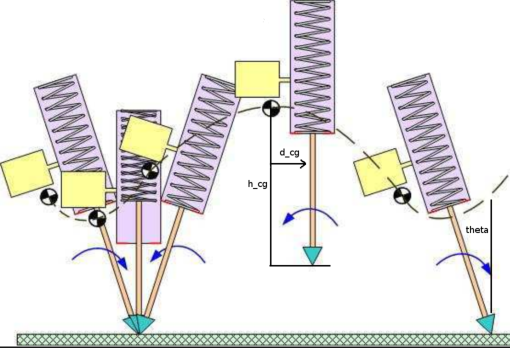
\includegraphics[scale = 0.8]{fig/slom_motion.pdf}
\label{schematic}
\end{figure}
Fig. \ref{schematic} shows the various stages in the motion of a \textit{Springy Leg Offset Mass} (SLOM) hopper. It consists
of a small leg mass attached to a large body mass with a spring. Energy is lost to the ground due to impacts of the
leg mass. If we can compensate this energy in every cycle using an Energy Pumping Mechanism (EPM), we can have a constant
hopping height. It is also seen that a
slight offset in the C.G. from the leg axis results in a stabilizing impulsive torque from the ground impact. Thus, while
running the robot tends to propel itself forward. 
A stable running gait is possible only for a specific value of the initial pitch and horizontal velocity. To remove this
constraint, we introduce
a reaction wheel for reorienting the hopper in mid-air. This is the Reaction Wheel Mechanism (ReWac). This project aims to build
a prototype of a SLOM one legged hopper and its reaction wheel mechanism to demonstrate a stable 2D hopping gait.\\

\section{Previous approaches}
Previous literature on this subject shows a vast array of actuation and stabilization methods. Notable among them are Marc Raibert's
pneumatically actuated Monopods, Beuhler's ARL Monopod's using ball and screw mechanism to store energy in a compression spring using
a motor and Zeglin's Bow Legged hopper which used an elastic carbon fibre element as a flexible leg to store energy.
On the other hand, for stabilization methods, we have hydraulically actuated hip in Raibert's Monopod and the compensatory winch
operated hip on the ARL Monopod I.\\

A prototype of SLOM hopper consists of a leg connected to the main body by a compression spring. A motor is used to compress
this spring to store
energy. The leg travels in and out of the main body and weighs almost $2/3^{rd}$ of the total mass of robot. This coupled with
the constant rubbing of the spring against its housing results in large frictional and impact loses.\\

Simit Pradhan developed a constraining mechanism for the SLOM hopper on a treadmill. He demonstrated a feed-forward controller
to control the hopping height. Siraj Issani has worked on the reaction wheel reorientation by modeling a reaction wheel
pendulum as the hopper in mid-air.\\

This project aims to design an EPM using extension springs and a motor. The hopper will also consist of a reaction wheel.
An onboard embedded platform including motor drivers and an inertial measurement unit will be developed to control the robot.
2D running gait will be demonstrated using this new design at the end of the project.\\

\section{Mechanical Design}
\subsection{Design 1}
This consists of a platform (body mass M) hanging around the leg (m) using an extension spring. A motor attached to the platform
pulls the platform downwards while winding to store energy in the springs. A constraint mechanism was designed for the platform
so that the motor does not need to provide continuous torque after satisfactory extension. An innovative mechanism to utilize
the wasted impact forces to release this constraint mechanism (thus resulting in release of stored energy in the spring) was
designed. A reaction wheel is positioned on the platform to provide an offset mass as well as for reorientation. This design has
a few problems associated with the winch of the motor. Also, the motor has to rotate in the opposite direction to unwind the winch.
The motor will have to free the winch faster than the compression of the spring.

\subsection{Design 2}
A second design used a rack positioned on the leg for the EPM. A dual shaft motor is attached to a worm-worm wheel configuration
to travel along the rack and extending the springs connected to the platform in the process. The other end of the shaft consists of
a friction pulley which forms the constraint mechanism along with a band drive connecting the platform and the leg together. The
constraint mechanism of this design is not satisfactory and has to be looked into.

\section{Choosing components}
Three major areas of operation such as the EPM, ReWac and hopping frequency modes were studied to decide the range of admissible
values for the masses, DC motors and electronic components.
\subsection{EPM}
An analysis of energy losses due to impact was done to decide the required extension in springs. Equations for rack-worm wheel-worm
system were used to translate the spring force and extension into a required torque and omega for the motor. This was used to
decide on the part numbers of the motor and the gear box. We also get an idea of the values of M and m using this analysis.
\subsection{ReWac}
We want to achieve reorientation for a running gait within one hop after the hopper has been started in an arbitrary initial
condition. We take the initial condition as a vertical drop from height H and try to reorient the resultant negative pitch into
an arbitrary positive pitch within one hopping cycle. Torque coupling between the reaction wheel and the body is solved to obtain
omega and torque for the ReWac motor which is used to select the motor and the gear-box.
\subsection{Hopping Frequency}
Desired hopping height dictates the hopping frequency. It is noted that if this matches with the natural frequency of the system,
there are large impact energy loses. We want to separate the two frequencies as much as possible to ensure that there is no resonance
condition even for small hopping heights. We analyze this problem to put bounds on the maximum leg mass (m).\\

\section{Embedded System}
Microchip dsPIC33F micro-controller is used for the onboard platform. A previously developed board using this, a motor driver,
an accelerometer and a gyroscope was used for experimentation. There is provision to obtain telemetry using XBee wireless
trans-receiver modules. We choose
digital inertial sensors over analog ones as they are pre-calibrated and more accurate even though they are usually only single axis
sensors. The TCM constraint designed by Simit ensures that we only need to sense the pitch of the robot.
\subsection{Kalman Filter}
A Kalman filter was developed to fuse data from the accelerometer and gyroscope to estimate $x = [ \theta\:\:\:\:\dot{\theta}]^T$.
A number of experiments were done on this to observe that it has good low frequency and high frequency response.
These experiments did not show any gyroscope bias in this sensor even after extended periods of operation.
We need to test this IMU for free-fall conditions. These conditions will be encountered for almost 30\% of the cycle time.
\subsection{Motor Control}
The micro-controller's quadrature encoder module (QEI) was used to obtain feedback of the motor velocity. This was used to get
a PID controller to follow a trapezoidal profile similar to the one we will use for both the EPM and ReWac motors.

\section{Future Work}
Fabrication of components will be done once the problems of the mechanical design are ironed out to get a satisfactory design.
The embedded system can be designed and tested meanwhile. Control strategies like the feed-forward controller for hopping height
and LQR controller for reorientation will be implemented. Integration of this system will be followed by testing and experiments
on a treadmill.
\end{document}
